\section{Episode 1: Riphard Begins}

Welcome to the world of Velterra, domain of the Seven, who rule over all from afar through the constant vigilance of the Church.

“In Hope’s Rest, the largest city of the Empire of the Seven, a cloaked man dashes over rooftops, a half-burnt tome tucked under one arm as a group of mercenaries chase him. Abruptly he comes to a dead end, a roof with nowhere to leap to and nowhere to hide. He turns to face his attackers and reaches for his weapons, the book slipping from his grasp as he does so. In a moment of panic he spins to grab for the book, losing his balance and toppling from the roof as the mercenaries swing their blades at his back.”

“In the north, a pair of goblin twins flee the perils of Valkar Varg’s reign, seeking the freedom and new life the south can bring. They are surrounded by brutal tribesmen and vicious axes on all sides, angered by their desertion. As the two goblins look at each other in desperation and anger they nod, the girl raising a long rifle that quivers with electricity, the boy raising a small hunting bow and quickly loosing several arrows. As their enemies close in the bow-user pulls a vial of some mysterious viscous liquid as his twin sister unclips a thrumming round device from her belt. In moments, a huge explosion rips through the area.”

“To the south, a dwarf pastor sits hunched over a tome, scribbling notes. He raises his head as he hears the slow creak of his door, aware that he is expecting no visitors. He stands and turns to see a hulking figure behind him, armoured with a long-barelled gun at his side. The dwarf rests a trembling hand on his holster as a man who should not exist stands before him. Terse words are exchanged, accusations and threats. The dwarf grits his teeth and sets his feet, drawing the pistol at his side as his opponent does the same. From outside, the sound of a single shot being fired can be heard.”

“To the East, a figure wrapped in cloth and strange garments sits quietly in a harbour tavern in Port Averdale, recently arrived on the continent from a long voyage. She sits with an untouched mug of unappealing ale in front of her as three thugs approach the table. They slam down a parchment on the table with a picture and a hefty figure. In a flash she is to her feet, blade drawn and two of the men sliced apart on the ground. She faces the remaining thug who whistles and a stream of men pour into the building from all around. Outnumbered by scores and with a demand the surrender, she chooses the only option she knows. Honour.”

A group of strangers meet up in a featureless, polished stone room, none fully understanding what has brought them there. An elephantine creature (Meredith) beckons them through a mysteriously appearing door into a plush office where a red skinned man wearing a human face mask welcomes them.

The man explains that he is called Lazarus and that the group have all recently died. They have been brought together, here, and given a second chance at life in exchange for carrying out a mission to destroy the Church Upon asking for proof Pilch is shown the full, gory reality of their situation through a window into hell Lazarus explains that the group must obtain the Stone of Anthala from the temple of XXX and our given basic directions. This ancient relic will be the source of future communications with Lazarus and his means of issuing further instructions. They are warned not to gain the attention of the Church.

The group agree to carry out the task and are transported into a cavern, where winter clothes and supplies await them. After some brief introductions Exme opens the cave door to reveal they are in a snowy wilderness The group spend two days walking South (Kolo relieves Pilch of 15 gp during the trip) until they reach the town of Vathos Boundary. During a surprise fight with some wolves the two goblins disappear. Riphard finds that his gun has become faulty but is able to restore it to proper working order with a good clean.

The remaining members enter the town, Pilch in disguise, and go about making inquiries. Riphard and Ontario make a visit to a local smith, not Gerard, who is able to sell bullets and black powder. Onatrio gets the lay of the land, and discovers that the locals are fine with the Church.

The two goblins, desperate to perform their own investigation and disguised as a single person in an overcoat, put Pilch’s money to work inebriating an entire titty bar, whilst loudly exclaiming their adventurous intentions. Otoria witnesses a man being beaten to death in the street.

Several towns folk inform the party about the dreaded masked “tikk-tukks” that lie to the South of the town, these are small bear like creatures with face masks.

The party is reunited in the titty bar. After a brief altercation between Kolo and Pilch concerning some mislocated funds, Exme and Riphard discuss the finer points of owning firearms and Esme is thrilled to get her first real look at a Church gun.

Ontario and Pilchard Meet a hunter named Gerard who gives a brief description of the location of the temple of Anthala lost in the south. Kolo discovers more about what eats people, and gives Pilchs name as a point of contact. Due to the incredible generosity of Pilch’s money, the group are offered free board at the titty bar and take the opportunity to rest up.

The next day they make their way out of town. As they leave, an explosion rips through the local stable, decimating several horses and destroying the building. Riphard is unable to identify the source of the explosion, however Kolo is quick to demonstrate the kindness and superiority of Goblin-folk by using the rest of Pilch’s money to compensate the stable owner for the damage. Along with casting wild aspersions to the gathered crowd as to who might be the culprit, ie only group who has access to black powder (Church).

The group make their way south to the temple

\begin{center}
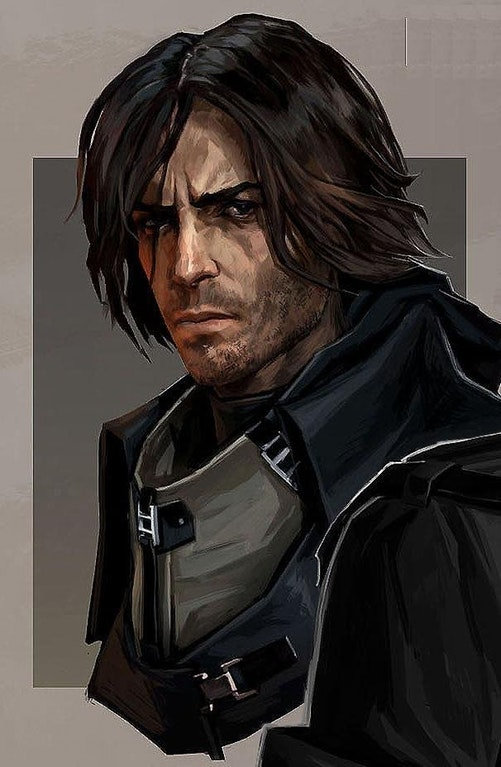
\includegraphics[width=80mm]{./img/pilch1.jpg}
\begin{figure}[h]
\end{figure}
\end{center}

\clearpage